\chapter{Natural Language Processing (NLP)}
Il \textbf{Natural Language Processing} (NLP) si occupa di studiare il linguaggio
naturale introducendo la semantica e le relazioni tra le parole. Oltre a questo,
si occupa di analizzare il testo, capire il contesto ed estrarre varie informazioni,
partendo dai topic fino ad arrivare alle emozioni.

In NLP la parte fondamentale è trovare una rappresentazione delle parole. Questo
non è una cosa banale in quanto:
\begin{itemize}
      \item Ci serve un contesto per rappresentare il testo in analisi.
      \item Ci può essere del rumore nei dati (dati errati o non fedeli).
      \item Può essere presente dell'ambiguità nelle frasi, per esempio abbiamo
            modi di dire. Questo viene risolto in diversi modi, ad esempio
            effettuando l'analisi sintattici, part-of-speech tagging, etc.
      \item Ambiguità sintattica, la quale viene risolta attraverso part-tree-disambiguation
\end{itemize}
I problemi legati all'ambiguità sono molto importanti in questo campo, e sono
studiati in modo approfondito. Per la loro risoluzione esistono diverse tecniche
che sono state sviluppate nel tempo e implementate in librerie.
Alcune di queste, forniscono sistemi per risolvere le ambiguità nelle frasi, i
quali si basano sulla costruzione di diversi alberi di parsing e restituiscono
l'albero della frase più probabile.

Tra le varie tipologie di ambiguità che possiamo incontrare distinguiamo due
tipologie:
\begin{itemize}
      \item Ambiguità emozionale: in una frase sono espresse emozioni contrastanti.
            Questo viene studiato attraverso la \textbf{sentiment analysis}.
      \item Ambiguità semantica: in una frase sono presenti parole che possono
            avere più significati. Questo viene studiato attraverso la
            \textbf{named-entity recognition} e in seguito il \textbf{named-entity
                  linking}.
\end{itemize}
\section{Sentiment analysis}
\begin{definizione}[\textbf{Text Analytics}]
      La \textbf{text analytics} è una tecnica che permette di estrarre informazioni
      dal linguaggio naturale per identificare informazioni soggettive e oggettive.
\end{definizione}
La fase di analisi consiste nel classificare il testo in base al fatto che esso
sia:
\begin{itemize}
      \item \textbf{Oggettivo}: si sta esprimendo un fatto.
      \item \textbf{Soggettivo} (emozione): si sta esprimendo un'emozione la quale
            può essere:
            \begin{itemize}
                  \item Positivo.
                  \item Negativo.
                  \item Neutrale: complesso perché spesso è molto vicino ad una
                        frase oggettiva o spesso si pesa la frase tra positiva e
                        negativa, quindi se è bilanciata è neutrale.
            \end{itemize}
\end{itemize}
Un'altra distinzione che possiamo fare è tra:
\begin{itemize}
      \item \textbf{Esplicito}: il testo esprime chiaramente un opinione.
      \item \textbf{Implicito}: il testo esprime un opinione in modo indiretto.
\end{itemize}
Un altro problema di riconoscere il sentiment è capire se nella frase è
presente dell'ironia o del sarcasmo.
\begin{definizione}
      Le emozioni sono un fenomeno psicologico che viene azionato da stimoli
      culturali oppure da esperienze passate. Esse possono essere:
      \begin{itemize}
            \item Rabbia
            \item Disgusto
            \item Paura
            \item Felicità
            \item Tristezza
            \item Sorpresa
      \end{itemize}
      Esiste una diversa classificazione, la quale le rappresenta con 8 emozioni
      graduali.
      \begin{figure}[!ht]
            \centering
            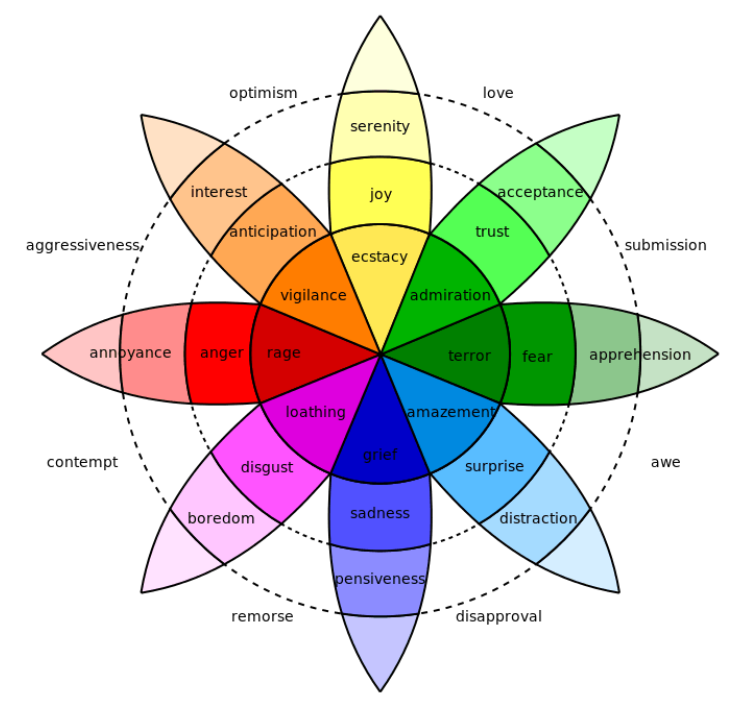
\includegraphics[width=0.5\textwidth]{./img/nlp/emozioni.png}
            \caption{Classificazione delle emozioni}
            \label{fig:emozioni}
      \end{figure}
\end{definizione}
\subsection{Rappresentazione del testo}
Il primo passo consiste nel capire come rappresentare il testo. Questo passaggio
è necessario per passare da una misura qualitativa a una misura quantitativa.

Una prima soluzione è quella di rappresentare il testo tramite un dizionario
di parole. Questo metodo è molto semplice e permette di rappresentare il testo
come un vettore di bit, dove il bit $i$-esimo è a $1$ se la parola $i$-esima
è presente nella frase. Questo metodo però ha dei problemi:
\begin{itemize}
      \item Il vettore che rappresenta la frase è molto grande e sparso.
      \item Perdiamo l'ordinamento delle parole.
\end{itemize}
Un ulteriore metodo è rappresentato dalla \textbf{BagOfWord}, la quale consiste
nel rappresentare una frase tramite un vettore in uno spazio. Il problema è che
manca la composizionalità delle parole.

Possiamo usare una rappresentazione deep basata su \textbf{word2vec}. Questa consiste
nello scrivere il termine sulla base dei termini che lo precedono e che lo seguono.
Si ha quindi uns strategia simile alla BagOfWord, ma mantenendo la composizionalità.

Word2Vec è un modello che viene usato per creare una rappresentazione vettoriale
delle parole. Questo modello è basato su una rete neurale che prende in input
una parola e cerca di prevedere le parole che la circondano.
\begin{itemize}
      \item \textbf{skip-gram}: parte da una parola del documento e cerca di
            predire l'intorno della parola.

            Per ottenere questo risultato, usiamo un \textbf{one-hot-vector},
            ovvero un bitvector, lungo quanto il il vocabolario, con un bit a $1$
            nella posizione associata alla parola all'interno del vocabolario.

            Successivamente costruiamo una rete neurale (Encoder Decoder) che
            preso in input il bitvector, in output dobbiamo avere un vettore
            lungo tanto quanto il vocabolario con una probabilità associata ad
            ogni parola. La rappresentazione vettoriale coincide con  quello che
            si ha nell'hidden layer, la sua dimensione è decisa in fase di
            costruzione della rete.

            Il documento viene rappresentato dal vettore media dei vettori dei
            termini presenti nel documento.

            A differenza dalle rappresentazioni più vecchie abbiamo un vettore di
            dimensione $n$ selezionato dalla rete. Il problema è che non consideriamo
            il contesto del mondo.

            Esistono metodi più efficaci per rappresentare il testo come
            \textbf{USE} e \textbf{BERT}.
      \item \textbf{CBOW}: cerca di predire la parola sulla base dell'intorno
            delle parole vicine.
\end{itemize}
Questi permettono di avere parole con lo stesso significato o simili vicine nello
spazio vettoriale.

Una volta risolto il problema della rappresentazione si può passare alla fase
di classificazione. Questa può essere fatta in diversi modi:
\begin{itemize}
      \item \textbf{Lexicon-based}: si basa su un dizionario di parole associate
            a delle emozioni. Si contano le parole associate alle emozioni e si
            restituisce l'emozione con il conteggio maggiore. Se le emozioni hanno
            lo stesso numero di parole allora la frase è neutra.
      \item \textbf{Machine Learning}: si basa su un modello di classificazione
            che prende in input il vettore che rappresenta la frase e restituisce
            l'emozione.
\end{itemize}
\begin{nota}
      Nel primo caso risulta importate scegliere bene il lessico, perché le parole
      possono essere positive o negative in base al contesto.
\end{nota}

\section{Name entity recognition}
(disambiguazione dal punto di vista morfosintattico)
Uno dei tanti problemi è la disambiguità dei nomi di entità, quindi capire a che cosa 
si riferisce un entità, ovvero disambiguità delle entità che si trovano nei messaggi.
Per fare ciò si devono riconoscere i token delle entità e si deve capire a cosa si 
riferiscono.

I problemi nel riconoscere i token sono:
\begin{itemize}
      \item linguaggio rumoroso, ambiguità e polisemia
      \item out of vocabulary quando il modello non ha mai incontrato delle parole 
      che sta analizzando. Se io ho dato in fase di training The Big Bang Theory
      ma incontra TBBT, allora non lo riconosce.
      \item Out of Knowledge base quando il modello non ha una rappresentazione dell'entità nella 
      base di conoscienza.
\end{itemize}


L'entità vengono rappresentate come surface form, ovvero la loro rappresentazioen 
indipendente dalla semantica nella frase. Riconoscere un'entità si occupa di 
ricercare degli insiemi di token che poi vengono segmentati per in classi o etichette.
Ex: luoghi\dots.
Ora si usano modelli neurali che si basano su modelli di sequence prediction.
Ovvero si ha una sequenza di osservazioni e si impara per prevedere la sequenza 
ottimale di etichette. In questo modo si considera nella predizione il contesto 
delle osservazioni facenti parte della sequenza, quindi non si effettua il traning 
sulle singole parole.

Ora si utilizzano i Conditional Random Fields. Sono modelli grafici probabilistici 
che massimizzano la probabilitùà condizionata di etichette della sequenza di input.
Le osservazioni sono le parole, mentre gli stati nascosti sono le etichette.
Il modello associa una dipendeza tra la classe e la sua parola di input, inoltre 
si ha una dipendenza temporale solo con la parola precedente. (catene markoviane del 
primo ordine).

In fase di trainig si impara $P(y|x)$, $y$ vettore delle etichette dato $x$ vettore 
delle parole.

$$P(y|x) = \frac{1}{Z_x} \prod_t \phi(y_t,y_{t-1},x ,t)$$

dove $ \frac{1}{Z_x}$ costante di normalizzazione e $\phi(y_t,y_{t-1},x ,t) = \exp (\sum_k\lambda_k f_k(y_t,y_{t-1},x,t))$.
$f_k(y_t,y_{t-1},x,t)$ sono delle feature con function (predeterminate, a  valori reali e almento a 2 stati di uscita), 
valutano diverse proprietà in base all'osservazione, l'etichetta e l'etichetta precedente al tempo $t$.
Sono come degli if che valutano le caratteristiche del testo e le associano alle etichette 
sia della parola pattuale sia di quella precedente. Le feature function possono essere di tipo:
\begin{itemize}
      \item \textbf{state} $f_i$: valutano lo stato in cui ci si trova in quel tempo.
      Misurano la relazione $x_t$ e $y_t$
      \item \textbf{transizioni} $g_i$: modellano la dinamica dell'etichettatura.
      Misurano la relazione tra le label della parola attuale e quelle adiacenti. 
      Le definisco a runtime perché si applicano alle etichette.
\end{itemize} 

Il modello è un modello logaritmico lineare, quindi la composizione delle feature 
si effettua attraverso una somma, rimuovendo la produttoria. Dobbiamo imparare 
le $\lambda_i, \mu_j$, per fare ciò si massimizza la verosimiglianza del modello 
rispetto alle osservazioni.

L'inferenza consiste nel determinare la migliore sequenza di etichette data una 
sequenza di osservazioni. La rete del modello è una feed forward e sugli archi ci 
sono i pesi delle features function.

La valutazione del modello si effettua in due metodologie:
\begin{itemize}
      \item exact match: considero corretta la predizione se l'entità viene riconosciuta 
      correttamente. Utile se devo fare sentiment analisis. 
      \item partial match: considero corretta la predizione se l'entità viene riconosciuta 
      parzialmente. Utile se devo fare retrival del db.
\end{itemize}

Una volta riconosciuta l'entità spesso si effettua named-entity linking.
Ovvero utilizziamo l'etichetta per cercare l'informazione nelle basi di conoscienza,
l'etichetta diventa un criterio di selezioni o una probabilità a priori.

\section{Word sense disambiguation}
Si cerca di comprendere il significato della parola accettato comunemente. è un 
task importante perché permette di disambiguare dal punto di vista del senso.

Il problema è che il significato può essere dedotto da quelle adiacenti.

Gli approcci sono:
\begin{itemize}
      \item basati su basi di conoscienza: si usano risorse lessicali come 
      dizionari e tesauri
      \item supervisionati
      \item non supervisionati
\end{itemize}

Nei metodi basati su basi di conoscienza, la disambiguazione della parola si effettua 
tramite un dizionario machine readable e dati raw. Non servono dati etichettati e 
si lavora su parole appartenenti alle open class. Nei dizionari si possono trovare 
significati, definizioni ed esempi utili per disambiguare.

Un primo algoritmo è Lesk algorithm, definisce il senso delle parole nel contesto
confrontando le definizioni si sovrapposizioni. In sostanza:
\begin{itemize}
      \item prende tutti i significati di tutte le parole da disambiguare
      \item determina gli overlap tra tutte le coppie di parole da disambiguare
      \item seleziona il significato in base al massimo numero di overlap.
\end{itemize}
Algoritmo naive molto pesante.

è stato introdotto Simplified Lesk che misura l'overlap del significato di una 
parola e tutte quelle del contesto da disambiguare. Quindi non si hanno più combinazioni 
ma si confronta i significati di una sola parola alla volta rispetto a tutte le
altre.